\documentclass[a4paper]{exam}
\usepackage{amsfonts,amsmath,amsthm}
\usepackage[a4paper]{geometry}
\usepackage{xcolor}
\usepackage{wasysym}


\usepackage{amsfonts,amsmath,amsthm}
\usepackage{xcolor}
\usepackage{wasysym}

\usepackage{tikz}
\usepackage{tikz-qtree}

\newtheorem{definition}{Definition}

\newcommand\N{\ensuremath{\mathbb{N}}}
\newcommand\union{\cup}
\newcommand\interx{\cap}

\header{CS/MATH 113}{WC11: Graph Isomorphism}{Spring 2025}
\footer{}{Page \thepage\ of \numpages}{}
\runningheadrule
\runningfootrule

% \printanswers

\qformat{{\large\bf \thequestion. \thequestiontitle}\hfill}
\boxedpoints

\title{Weekly Challenge 11: Graph Isomorphism}
\author{CS/MATH 113 Discrete Mathematics}
\date{Spring 2025}

\begin{document}
\maketitle




\begin{questions}
    \titledquestion{Breaking things down}[10]
    \begin{definition}
        Let $G = (V,E)$ be a graph. A decomposition of $G$ is a list of subgraphs of $G$ (obtained from removing edges of $G$) such that each edge appears in exactly one subgraph in the list.
    \end{definition}

    \begin{figure}[!h]
        % \vspace*{1cm}
        \begin{center}
        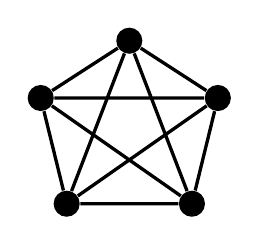
\begin{tikzpicture}[scale=.75]
            
            \node[style={fill=black,circle}] (a) at (4,1.7){};
            \node[style={fill=black,circle}] (b) at (2.5,0.73){};
            \node[style={fill=black,circle}] (c) at (2.939339828,-1.06){};
            \node[style={fill=black,circle}] (d) at (5.06066,-1.06){};
            \node[style={fill=black,circle}] (e) at (5.499,0.73){};
            \draw[black,very thick] (a)--(b) (a)--(c) (a)--(d) (a)--(e) (b)--(c) (b)--(d) (b)--(e) (c)--(d) (c)--(e) (d)--(e);
    
            \end{tikzpicture} 
            \hspace{1cm} \includegraphics[scale = 0.1]{right-arrow.png} \hspace{1cm}
            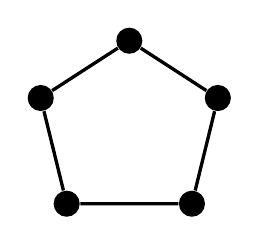
\begin{tikzpicture}[scale=.75]
            
                \node[style={fill=black,circle}] (a) at (4,1.7){};
                \node[style={fill=black,circle}] (b) at (2.5,0.73){};
                \node[style={fill=black,circle}] (c) at (2.939339828,-1.06){};
                \node[style={fill=black,circle}] (d) at (5.06066,-1.06){};
                \node[style={fill=black,circle}] (e) at (5.499,0.73){};
                \draw[black,very thick] (a)--(b) (a)--(e) (b)--(c)  (c)--(d) (d)--(e);
        
                \end{tikzpicture} 
                \hspace{1cm}
                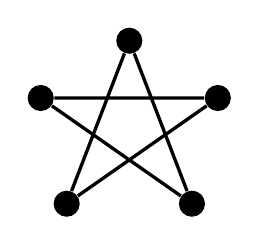
\begin{tikzpicture}[scale=.75]
            
                    \node[style={fill=black,circle}] (a) at (4,1.7){};
                    \node[style={fill=black,circle}] (b) at (2.5,0.73){};
                    \node[style={fill=black,circle}] (c) at (2.939339828,-1.06){};
                    \node[style={fill=black,circle}] (d) at (5.06066,-1.06){};
                    \node[style={fill=black,circle}] (e) at (5.499,0.73){};
                    \draw[black,very thick]  (a)--(c) (a)--(d) (b)--(d) (b)--(e) (c)--(e) ;
            
                    \end{tikzpicture} 
        \end{center}
            \caption{An example of decomposition of $K_5$ into two $C_5$s.}  
            \label{fig:exampl_ahg}     
    \end{figure}
    
    Prove that for any $n\in \mathbb{Z}^+\setminus\{1,2\}$ the graph $K_n$ can be decomposed into three isomorphic subgraphs if and only if $n+1$ is not divisible by 3. 
    \begin{solution}
        % Enter solution here
    \end{solution}

    \titledquestion{Reviews}[0] How was CS/Math 113? Did you enjoy the course? what was your favorite and what was your lease favorite part of the course. Please let us know if you have any suggestions for future iterations of this course.
    \begin{solution}
        % Enter solution here
    \end{solution}

    \titledquestion{Healing}[0] Go outside take a deep breath and get 8 hours of sleep tonight.
    \begin{solution}
        % Enter solution here
    \end{solution}
    
\end{questions}

\end{document}
%%% Local Variables:
%%% mode: latex
%%% TeX-master: t
%%% End:


